%\chapterauthor{Author Name}{Author Affiliation}
%\chapterauthor{Second Author}{Second Author Affiliation}
\chapter{Text File Editing} \label{ch:tfe}

Many text editors are supported in Linux, to name a few, Vim, Emacs, gedit, Visual Studio Code. These text editors come with different features. Some of the text editors even provide integrated development environment for a large set of programming languages.

Among the vast number of choices, Vim and its variations are probably the most popular text editors. Vim works perfectly in a shell environment without relying on graphical desktops, thus is adopted by many Linux distributions as the built-in default text editor. NeoVim is a popular fork of Vim, and it is introduced briefly in the end of the chapter. The majority of features introduced about Vim also apply to NeoVim.

\section{General Introduction to Vim}

\mync{Vi IMproved}[Vim] is a free and open-source software developed by Bram Moolenaar et al. It is an expansion to the Vi text editor to include features such as syntax highlighting, etc., and has become the default text editor of many Unix/Linux based operating systems.

Bram Moolenaar, the original inventor of Vim, passed away on August 3, 2023 at the age of 62. His project Vim has been taken over by the contributors from the community. 

\subsection{Main Features}

Some people claim Vim to be the most powerful text file editor and \myabb{Integrated Development Environment}{IDE} for programming on a Linux machine (and potentially on all computers and servers). The main reasons are as follows.
\begin{itemize}
  \item Vim is usually built-in to Linux during the operating system installation, making it the most available and cost-effective text editor.
  \item Vim can work on machines where graphical desktop is not supported. It is light in size and is suitable to run even on an embedded system.
  \item Vim operations are done mostly via mode switching and shortcut keys without requiring mouse movement, and hence the operation efficiency can be improved.
  \item Vim is highly flexible and can be customized according to the user's habit, and can be integrated with third-party tools (for example, GitHub Copilot) which boost its capability.
\end{itemize}

Vim can become very powerful and convenient for the user if the user becomes proficient with it. However, Vim is not as intuitive as other text editors with graphical interfaces, and there might be a learning curve for the beginners.

\subsection{Vim Modes} \label{ch:tfe:subsec:vimgeneralintro}

Unlike other text editors, Vim defines four different modes, namely \mync{normal mode}, \mync{insert mode}, \mync{visual mode} and \mync{command line mode}, as summarized in Table \ref{ch:tfe:tab:vimmodes}.

\begin{table}[!htb]
  \centering \caption{Commonly used modes in Vim.}\label{ch:tfe:tab:vimmodes}
  \begin{tabularx}{\textwidth}{lX}
    \hline
    Mode & Description \\ \hline
    Normal & Default mode. It is used to navigate the cursor in the text, search and replace text pieces, and run basic text operations such as undo, redo, cut (delete), copy and paste. \\ 
    Insert & It is used to insert keyboard inputs into the text, just like commonly used text editors today. \\ 
    Visual & It is similar to normal mode, and it allows the user to select a block of text. Normal mode commands can be used on the selected text. \\ 
    Cmdline & It takes in a single line command input and perform actions accordingly, such as save and quit. \\
    \hline
  \end{tabularx}
\end{table}

As a start, the following basic commands can be used to quickly create, edit and save a text file using vim. In home directory, start a shell and key in
\begin{lstlisting}
$ vim testvim
\end{lstlisting}
to create a file named ``testvim'' and open the file using Vim. Notice that in some Linux versions, Vi might be aliased to Vim by default.

In the opened file, use \verb|Esc| and \verb|i|/\verb|a| (insert/append) to switch between normal mode and insert mode. Notice that in the normal mode, the cursor is on a character. When using the insert command, the insertion cursor is put to the left of that character, whereas when using the append command, the insertion cursor is put to the right of that character. In the normal mode, use \verb|h|, \verb|j|, \verb|k|, \verb|l| to navigate the position of the cursor. If a modern keyboard is used, the left, right, up and down arrows can also be used to navigate the position of the cursor in both normal and insert modes. Finally, in the normal mode, use \verb|:w| to save the file, and \verb|:q| to quit Vim, or use \verb|:wq| to save and quit Vim.

The above basic commands and their relationships are summarized in Fig.~\ref{ch:tfe:fig:vimbasicmodeswitching}. A flowchart for creating/opening, editing, saving, and quitting a text file using the aforementioned commands is given in Fig.~\ref{ch:tfe:fig:vimbasicoperationflowchart}.

\begin{figure}[!htb]
\centering
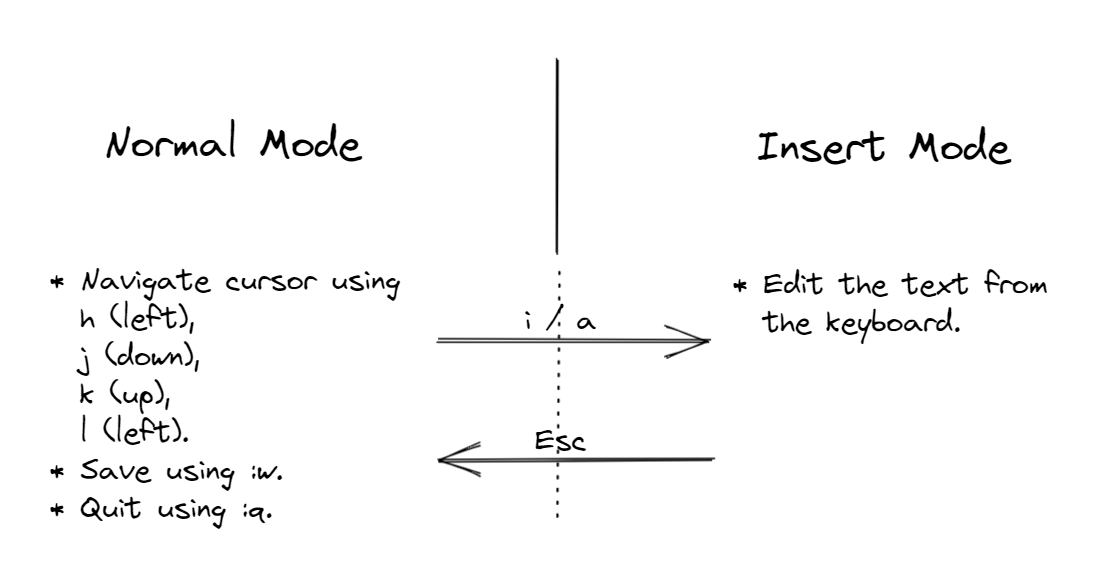
\includegraphics[width=250pt]{chapters/part-1/figures/vimbasicmodeswitching.png}
\caption{Mode switching between normal mode and insert mode, and basic functions associated with the modes.} \label{ch:tfe:fig:vimbasicmodeswitching}
\end{figure}

\begin{figure}[!htb]
\centering
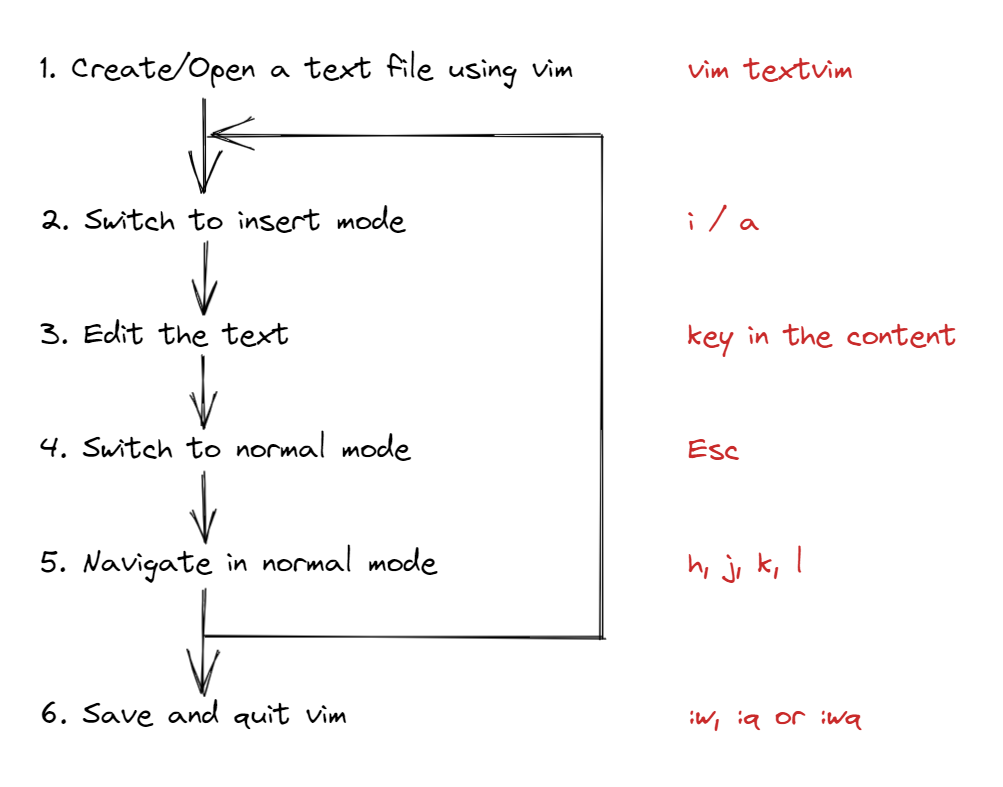
\includegraphics[width=250pt]{chapters/part-1/figures/vimbasicoperationflowchart.png}
\caption{A flowchart for simple creating, editing and saving of a text file using Vim.} \label{ch:tfe:fig:vimbasicoperationflowchart}
\end{figure}

There are other shortcuts that switch from normal mode to insert mode. Some of them are summarized in Table \ref{ch:tfe:tab:switchtoinsert}.

\begin{table}
  \centering \caption{Commonly used shortcuts to switch from normal mode to insert mode.}\label{ch:tfe:tab:switchtoinsert}
  \begin{tabularx}{\textwidth}{lX}
    \hline
    Operator & Description \\ \hline
    \verb|i| & Insert before the character at the cursor. \\ 
    \verb|I| & Insert at the beginning of the row at the cursor. \\ 
    \verb|a| & Insert after the character at the cursor. \\ 
    \verb|A| & Insert at the end of the row at the cursor. \\ 
    \verb|o| & Create a new row below the cursor and switch to insert mode. \\ 
    \verb|O| & Create a new row above the cursor and switch to insert mode. \\
    \hline
  \end{tabularx}
\end{table}

\section{Vim Customization}

With the basic operations introduced in Section \ref{ch:tfe:subsec:vimgeneralintro}, we are able to create and edit text files of any kind. Though at this point the advantages of using Vim over other text editors are not obvious yet, the Vim editor is at least useable.

We can now customize the user profile for better user experience. Notice that the customization is completely optional and personal. This section only introduces the idea and basic methods such as re-mapping keys and creating user-defined shortcuts. Everything introduced here are merely examples and it is completely up to the user how to design and implement his own profile.

In Linux, navigate to home directory. Create the following path and file \verb|~/.vim/vimrc| or \verb|~/.vimrc|, which will serve as the Vim configuration file. Each time Vim is started, it will automatically access this file and apply the configurations inside.

There are many readily available \verb|vimrc| profiles shared in the community. Feel free to use them as a reference when creating a new one.

\subsection{Shortcuts}

It is desirable to re-map some keys to speed up the text editing. For example, by mapping \verb|jj| to \verb|Esc| in insert mode, one can switch from insert mode to normal mode quickly (notice that consequent ``jj'' is rarely used in English). The mapping of keys and keys combinations can be done as follows in \verb|vimrc|.
\begin{lstlisting}
inoremap jj <Esc>
\end{lstlisting}
where \verb|inoremap| is used to map keys (combinations) in insert mode (and \verb|noremap| in normal and visual modes).

The upper case letter \verb|S| and lower case letter \verb|s| in normal mode are originally used to delete and substitute texts, and they are rarely used due to the more powerful shortcut \verb|c| which does similar tasks. We can re-map \verb|S| to saving, and disable \verb|s|. Similarly, upper case letter \verb|Q| is mapped to quitting Vim.
\begin{lstlisting}
noremap s <nop>
map S :w<CR>
map Q :q<CR>
\end{lstlisting}
where \verb|<nop>| stands for ``no operation'' and \verb|CR| stands for the ``enter'' key on the keyboard. The keyword \verb|map| differs from \verb|noremap| in the sense that \verb|map| is for recursive mapping.

\subsection{Syntax and Color Scheme}

By default Vim displays white colored contents on a black background. Use the following command in \verb|vimrc| to enable syntax highlighting or change color schemes. Use \verb|:colorscheme| in cmdline mode in Vim to check for available color schemes.
\begin{lstlisting}
syntax on
colorscheme default
\end{lstlisting}

The following setups in \verb|vimrc| displays the row index and cursor line (a underline at cursor position) of the text, which can become handy during the programming. Furthermore, it sets auto-wrap of text when a single row is longer than the displaying screen.
\begin{lstlisting}
set number
set cursorline
set wrap
\end{lstlisting}

The following command opens a ``menu'' when using cmdline mode, making it easier to key in commands.
\begin{lstlisting}
set wildmenu
\end{lstlisting}

\subsection{Scrolling}

Use \verb|scrolloff| to make sure that when scrolling in Vim, there are always margins lines in the top and bottom of the screen, so that the cursor is always close to the centre of the screen.
\begin{lstlisting}
set scrolloff=3
\end{lstlisting}

\subsection{Spell Check}

Enable spell check in Vim as follows.
\begin{lstlisting}
map sc :set spell!<CR>
\end{lstlisting}
where \verb|sc| can be used to quickly turn on and off the spell check function. In addition, when the cursor is put on the wrongly spelled word, use \verb|z=| to open a list of possible corrections.

\subsection{Search Highlight}

The following customization in \verb|vimrc| shall give a better searching experience. When searching in the text for a particular word or phrase (more about searching in the text will be introduced in later sections), to make the search results highlighted, add the following line to the user profile \verb|vimrc|.
\begin{lstlisting}
set hlsearch
exec "nohlsearch"
set incsearch
noremap <Space> :nohlsearch<CR>
set ignorecase
noremap = nzz
noremap - Nzz
\end{lstlisting}
where \verb|hlsearch| enables highlighting all matching results in the text, and \verb|incsearch| enables highlighting texts along with typing the keyword. 

Vim remembers the keyword from the previous search and may automatically highlight them in the text on a new session. This can be confusing sometimes. To tackle the issue, use command \verb|exec "nohlsearch"| (\verb|exec| in \verb|vimrc| executes a command when starting a new session) after \verb|set hlsearch| to force Vim to clear its searching memory on a new session. 

To quit searching, use \verb|:nohlsearch| in cmdline mode. For convenience, consider mapping it with a customized shortcut key such as \verb|Space|. 

Set \verb|ignorecase| to ignore case-sensitive during the searching.

Keys \verb|n| and \verb|N| are used to navigate through the search results, and \verb|zz| is used to center the cursor position on the screen. For convenience, they are mapped to \verb|=| and \verb|-|.

\subsection{Screen Splitting}

Screen splitting and resizing can be done in command line mode, and more details are introduced in the remainder of the chapter. Useful mappings are given below.

Use \verb|:split| and \verb|:vsplit| for horizontal and vertical screen splitting, respectively. A second split window would show up with the same text file opened. For simplicity, these commands can be mapped in \verb|vimrc| as follows.
\begin{lstlisting}
noremap sh :set nosplitright<CR>:vsplit<CR>
noremap sl :set splitright<CR>:vsplit<CR>
noremap sk :set nosplitbelow<CR>:split<CR>
noremap sj :set splitbelow<CR>:split<CR>
\end{lstlisting}
where \verb|splitright| and \verb|splitbelow| is used to setup the default cursor position after splitting the screen.

In a split window, open a new file using \verb|:e <path>|. To navigate the cursor across different split windows, use \verb|Ctrl+w| followed by \verb|h|, \verb|j|, \verb|k| and \verb|l|. For simplicity, they can be mapped as follows.
\begin{lstlisting}
noremap <C-h> <C-w>h
noremap <C-l> <C-w>l
noremap <C-k> <C-w>k
noremap <C-j> <C-w>j
\end{lstlisting}
where \verb|<C->| stands for \verb|Ctrl+|.

Resize the selected split window using \verb|:res+<number>|, \verb|:res-<numer>|, \verb|:vertical resize+<number>|, \verb|:vertical resize-<number>|. For simplicity, map these commands as follows.
\begin{lstlisting}
noremap H :vertical resize-2<CR>
noremap L :vertical resize+2<CR>
noremap K :res+2<CR>
noremap J :res-2<CR>
\end{lstlisting}

\subsection{Plug Tool}

In the Linux community, many plug tools have been created to add useful features for Vim. As a demonstration, in this section \mync{vim-plug}, a light-size vim plugin management tool created on GitHub, is used to install selected Vim plugins. Details about vim-plug can be found at GitHub under \textit{junegunn/vim-plug}.

Following the instructions given by GitHub under \textit{junegunn/vim-plug}, to use vim-plug on Linux, the very first step is to use \verb|curl|, a command-line tool for transferring data specified with URL syntax, to download vim-plug. To install \verb|curl| on Red-Hat-based distributions, use
\begin{lstlisting}
$ sudo dnf install curl
\end{lstlisting}
and on debian-based distributions, use \verb|apt| instead of \verb|dnf|.

With \verb|curl| installed, use the following in the shell to install vim-plug
\begin{lstlisting}
$ curl -fLo ~/.vim/autoload/plug.vim --create-dirs \
    https://raw.githubusercontent.com/junegunn/vim-plug/master/plug.vim
\end{lstlisting}
In the very beginning of \verb|vimrc|, add the following to specify the plugins to be installed. As an example, \textit{vim-airline/vim-airline} and \textit{joshdick/onedark.vim} are to be installed, the first of which adds a status line at the bottom of the Vim window, and the second adds a popular color scheme ``onedark''.
\begin{lstlisting}
call plug#begin()
Plug 'vim-airline/vim-airline'
Plug 'joshdick/onedark.vim'
call plug#end()
\end{lstlisting}
Finally, reload \verb|vimrc|, then run \verb|:PlugInstall| in cmdline mode to install the plugins. Use \verb|colorscheme onedark| instead of \verb|colorscheme default| in \verb|vimrc| to enjoy the onedark color scheme.

Notice that instead of setting up configurations permanently in \verb|vimrc|, the user can also apply a setup in cmdline mode for temporary use in an open session. A full list of \verb|vimrc| configurations used in this chapter can be found in the appendix.

\section{Basic Operations}

This section introduces basic Vim operations in normal mode.

\subsection{General Rule}

Many Vim commands in normal mode follow a common pattern: an operator command directly followed by a motion command, without spaces in between. For some operators, the motion argument is mandatory. The pattern is shown below.
\begin{lstlisting}
<operator><motion>
\end{lstlisting}

The operator specifies the action (for example, delete, yank, or change), while the motion specifies the range to which the action applies (for example, a character, a word, a line, or the entire file). Some operators may work without an explicit motion, or they may have a default motion. 

For example, consider the \verb|u| command for undo. It is not an operator–motion command, but a standalone command that does not take a motion argument.

To repeat an operation multiple times, prepend the command with a number indicating how many times it should be executed.

\subsection{Delete, Cut, Copy and Paste}

Delete, cut, copy and paste are mostly done in normal mode as follows.

\vspace{0.1in}
\noindent \textbf{Quick Delete by Character}
\vspace{0.1in}

Use \verb|x| to delete the character at the cursor, or \verb|X| to delete the character before the cursor. To delete multiple characters, one option is to press \verb|x| or \verb|X| repeatedly (or hold the key). Alternatively, Vim allows automatic repetition by prefixing a count. For example, \verb|20x| deletes 20 characters starting from the cursor. The same principle applies to other operators and motions. For example, \verb|10l| moves the cursor 10 characters to the right.

\vspace{0.1in}
\noindent \textbf{Delete and Cut}
\vspace{0.1in}

In Vim, cutting text is equivalent to deleting it, since deleted text is stored in a register and can be pasted. Thus, all delete operations can be considered cut operations, and they are more flexible than simply using \verb|x| or \verb|X|.

The operator \verb|d| deletes text and it requires a motion to define the range. For example, \verb|dl| deletes one character to the right (the character at the cursor), while \verb|dh| deletes one character to the left. Similarly, \verb|d20l| deletes 20 characters to the right, where ``20l'' serves as the motion. A combination such as \verb|5d4l| also works, producing the same result as \verb|d20l|.

The operator \verb|d| becomes more powerful when combined with word motions. For example, \verb|w| is a word motion and its range is to the first character of the next word. Consider sentence ``William Shakespear (c. 23 April 1564[b] – 23 April 1616) was an English playwright, poet and actor.'' with the position of the cursor at ``S'' in ``Shakespear''. Operation \verb|dw| deletes ``Shakespear ''. When the cursor is in the middle of a word, \verb|dw| deletes from the cursor to the beginning of the next word. For instance, if the cursor is on the ``k'' in ``Shakespeare'', \verb|dw| deletes ``kespeare ''. Motion \verb|b| works similarly, except that it traces words backward to the left. To delete the whole word regardless of cursor position, use the ``inner word'' motion \verb|iw|. For example, \verb|diw| deletes the entire word under the cursor but keeps the following space.

In addition to character motions (\verb|h|, \verb|l|) and word motions (\verb|b|, \verb|w|), there are sentence motions \verb|(| and \verb|)|, and paragraph motions \verb|{| and \verb|}|. There are also ``inner'' motions such as \verb|is| (inner sentence), \verb|ip| (inner paragraph), \verb|i'|, \verb|i"|, \verb|i`| (inner quotations), and \verb|i(|, \verb|i<|, \verb|i{| (inner blocks). They all work in a similar manner.

\begin{table}[!htb]
  \centering \caption{Commonly used operators related to delete/cut, change, copy and paste.}\label{ch:tfe:tab:deletecut}
  \begin{tabularx}{\textwidth}{lX}
    \hline
    Operator & Description \\ \hline
    \verb|x| & Delete (cut) the character at the cursor. \\ 
    \verb|X| & Delete (cut) the character before the cursor. \\ 
    \verb|dd| & Delete (cut) the entire current line. \\ 
    \verb|d| & Delete (cut) text according to a motion. \\ 
    \verb|cc| & Change (replace) the entire current line. \\ 
    \verb|c| & Change text according to a motion. \\ 
    \verb|yy| & Copy (yank) the entire current line. \\ 
    \verb|y| & Copy (yank) text according to a motion. \\ 
    \verb|p| & Paste the most recently yanked or deleted text after the cursor. \\ 
    \hline
  \end{tabularx}
\end{table}

\begin{table}[!htb]
  \centering \caption{Commonly used motions.}\label{ch:tfe:tab:motion}
  \begin{tabularx}{\textwidth}{lX}
    \hline
    Motion & Description \\ \hline
    \verb|h|, \verb|l| & One character left or right. \\ 
    \verb|j|, \verb|k| & One line down or up. \\ 
    \verb|b| & Beginning of the current word, or the beginning of the previous word if the cursor is already at the beginning of a word. \\ 
    \verb|e| & End of the current word. \\ 
    \verb|w| & Beginning of the next word. \\ 
    \verb|(|, \verb|)| & One sentence backward or forward. \\ 
    \lstinline{\{}, \lstinline{\}} & One paragraph backward or forward. \\ 
    \verb|iw|, \verb|is|, \verb|ip| & Inner word, inner sentence, inner paragraph. \\ 
    \verb|aw|, \verb|as|, \verb|ap| & A word, a sentence, a paragraph (including trailing space or blank line). \\ 
    \verb|i(|, \verb|i<|, \verb|i[|, \verb|i|\lstinline{\}} & Inner block for different types of brackets. \\
    \verb|i'|, \verb|i"|, \verb|i`| & Inner quotation (single, double, backtick). \\ 
    \verb|0| (zero) & Beginning of the current line. \\ 
    \verb|$| & End of the current line. \\ 
    \verb|gg| & Beginning of the file. \\ 
    \verb|G| & End of the file. \\
    \hline
  \end{tabularx}
\end{table}

The operator \verb|c| works similarly to \verb|d|, except that it automatically switches to insert mode after removing the selected text. 

To copy text into a register, use \verb|y| (short for ``yank''), followed by a motion to indicate the range of text. The motions follow Table \ref{ch:tfe:tab:motion}. To paste the most recently yanked or deleted text after the cursor, use \verb|p|. No motion is required.

In addition to the motions listed in Table \ref{ch:tfe:tab:motion}, another commonly used type of motion is ``find by character.'' For example, consider the following line of text, with the cursor starting on the letter ``A'':
\begin{lstlisting}
ABCDEFG;HIJKLMN;OPQ;RST;UVW;XYZ
\end{lstlisting}

In normal mode, typing \verb|f| followed by a character moves the cursor to the next occurrence of that character on the same line. For example, \verb|fG| moves the cursor to the letter ``G''. Similarly, \verb|f;| moves the cursor to the first ``;'' after ``G''. Typing \verb|f;| again moves the cursor to the next ``;'' after ``N''. From there, \verb|2f;| moves the cursor to the ``;'' between ``T'' and ``U'', since it repeats the motion twice.

If the command \verb|df;| is used when the cursor is at the letter ``A'', Vim deletes everything from ``A'' through the first ``;'', resulting in the removal of ``ABCDEFG;''.

\subsection{Search in the Text}

In normal mode, use \verb|/<keyword>| followed by \verb|Enter| to search the file for a keyword. Keys \verb|n| and \verb|N| are used to navigate through the search results (\verb|n| repeats the search in the same direction, while \verb|N| reverses it). The command \verb|zz| recenters the current cursor line in the middle of the screen. 

When a search is active, \verb|n| and \verb|N| can also be used as motions together with delete, change, or yank (copy) operators, as shown in Table \ref{ch:tfe:tab:deletecut}.

\subsection{Other Commands}

Use \verb|Ctrl+o| and \verb|Ctrl+i| to jump backward and forward through the cursor position history, respectively. These commands only change the cursor position; they do not modify the text.

To perform a ``save as,'' use \verb|:w <new path>| in command-line mode.

In command-line mode, the prefix \verb|!| allows interaction with the shell. For example, consider the case of editing a read-only file when Vim was not started with \verb|sudo|. A simple \verb|:w| will fail. Instead, use:
\begin{lstlisting}
:w !sudo tee %
\end{lstlisting}
Here, \verb|tee| is a Linux command that takes standard input and writes it to a file, and \verb|%| refers to the current file.

Another example is inserting the contents of an external file into the current buffer. Move the cursor to the desired location, then use:
\begin{lstlisting}
:r !cat <filename>
\end{lstlisting}

\section{Visual Mode}

The use of a mouse makes selecting a block of text very intuitive. In most text editors, the selected text will be highlighted, as if the cursor expands from one character to the entire block of text. Sequentially, operations such as delete and copy can be performed on the selected text.

The three visual modes of Vim, namely \mync{visual (default)}, \mync{visual-line} and \mync{visual-block}, provide similar experience where the user can select and highlight a block of text.

Use \verb|v| to enter the visual mode, then navigate the cursor to select a block of text. This allows the user to select text between any two characters. An example is given by Fig. \ref{ch:tfe:fig:vimvm1}. Alternatively, use \verb|V| to enter the visual-line mode where multiple lines can be easily selected, and use \verb|<ctrl>+v| to enter visual-block mode to select a rectangular block of text.

\begin{figure}[htbp]
	\centering
	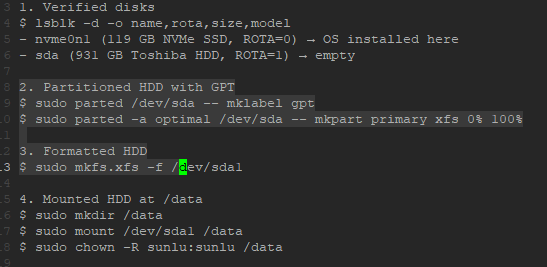
\includegraphics[width=0.8\textwidth]{chapters/part-1/figures/vimvm1.png}
	\caption{An example of visual mode where a block of text is selected.} \label{ch:tfe:fig:vimvm1}
\end{figure}

In any of the above visual mode, use \verb|:normal + <operation>| to execute operation(s) form the normal mode for each line. This allows convenient editing of multiple lines of text all together. For example, use \verb|V| to select a few lines of contents, followed by \verb|:normal 0iprefix-|. This will insert \verb|prefix-| to all the lines, as if \verb|0iprefix-| is executed in normal mode to all the lines separately, where \verb|0| (zero) navigates to the beginning of the line, \verb|i| switches to insert mode, and \verb|prefix-| is entered as the content.

Alternatively, in visual-block mode after selecting a block of content, use \verb|I| to enter insert mode and insert content in the first row of the selected block. When existing the insert mode using \verb|<Esc>|, the changes will apply to all selected rows. Similar effect can be achieved.

\section{Vim Macros}

\mync{Vim macros} allows the user to define a sequence of keyboard operations that can be recorded and triggered repeatedly. Use \verb|q| in normal mode to start and end a macro recording. The syntax follows
\begin{lstlisting}
q<macro-name><operations>q
\end{lstlisting}
where \verb|<macro-name>| is a single character that labels the macro.

Consider the following example where there is a text file containing the following content
\begin{lstlisting}
apple.jpg
pear.jpg
orange.jpg
banana.jpg
peach.jpg
\end{lstlisting}
and we would like to change the content to
\begin{lstlisting}
image: 'apple.jpg'
ttl: 5
image: 'pear.jpg'
ttl: 5
image: 'orange.jpg'
ttl: 5
image: 'banana.jpg'
ttl: 5
image: 'peach.jpg'
ttl: 5
\end{lstlisting}

In this example, repetitive work is involved and it is time consuming to do it manually if there are thousands of items in the file, and it is better to record a macro to automate the procedure. Navigate the cursor to the first row of the text, and type the following sequence of characters.
\begin{lstlisting}
q<macro name>0iimage: '<Esc>A'<Enter>ttl: 5<Esc>jq
\end{lstlisting}
where \verb|<macro name>| can be any character, for example \verb|s|. The string in the middle \verb|0iimage: '<Esc>A'<Enter>ttl: 5<Esc>j| is the necessary procedure to perform the revision for one row. If everything is done correctly, the file should appear as
\begin{lstlisting}
image: 'apple.jpg'
ttl: 5
pear.jpg
orange.jpg
banana.jpg
peach.jpg
\end{lstlisting}
and the cursor should be at row \verb|pear.jpg|.

To repeat the recorded procedures, use \verb|@<macro-name>|. In this example, just key in \verb|@s| in the normal mode, and the file should appear as
\begin{lstlisting}
image: 'apple.jpg'
ttl: 5
image: 'pear.jpg'
ttl: 5
orange.jpg
banana.jpg
peach.jpg
\end{lstlisting}

Repetitively using \verb|@s| proceeds with the revision. In the case the procedure needs to be repeated for many times, use \verb|<number>@<macro-name>|, in this example \verb|3@s|, to complete the remaining task.

\section{File Explorer and Screen Splitting}

Many IDEs come with project folder navigation and screen splitting features. In these IDEs, there is often a built-in file explorer, from where the user can navigate in the file system, select a file to edit, and the IDE will split the window for the selected file. Vim has similar features that supports file explorer and screen splitting, either via built-in functions or third-party support tools.

In Vim, use \verb|:Explore|, \verb|:Sexplore| or \verb|:Vexplore| (or \verb|:Ex|, \verb|:Sex|, \verb|:Vex| for short) in cmdline mode to open a file explorer, from where the user can navigate the cursor to select a file. Vim will then open the file in a split window that allows the user to further editing the file. There are many third-party plugin tools that enable convenient file explorer functions.

Use \verb|:split| and \verb|:vsplit| for horizontal and vertical screen splitting respectively. A second split window would show up with the same text file opened. Command \verb|splitright| and \verb|splitbelow| is used to setup the default cursor position after splitting the screen. To navigate the cursor across different split windows, use \verb|Ctrl+w| followed by \verb|h|, \verb|j|, \verb|k| and \verb|l|. Resize the selected split window using \verb|:res+<number>|, \verb|:res-<numer>|, \verb|:vertical resize+<number>|, \verb|:vertical resize-<number>|. 

\section{NeoVim}

Vim being an open-source project allows other to fork and build new projects on top of it. \mync{NeoVim} is one of those projects. Comparing with Vim whose code is almost all from Bram Moolenaar, NeoVim is more of a community-driven project with diversified contributors. 

A potential problem with project codes coming from a single contributor is that the code is often a bit more messy than if it were written and cross-checked by multiple contributors, and that has been the main criticism Vim has received. NeoVim, on the other hand, has cleaner code base. 

NeoVim is often regarded as a more cutting-edge version of Vim in the sense that new features usually come sooner in NeoVim than in Vim. NeoVim also has a better and more native support for Lua language. The configuration file for NeoVim, i.e., the counterpart of \verb|vimrc|, can be built by Lua files. Vim is initially a single-thread application, which is fine when it is used as a text editor. However, it limits the ability of Vim calling other shell services. The user needs to wait for the shell services to end before he can start editing the document again. NeoVim, on the other hand, uses multi-thread framework, hence does not pose this issue. Later on Vim added the support to allow plug-ins to trigger multi-thread processes.

The drawback of NeoVim is that it being a younger and more collaborative project seems to be less stable than Vim.

Both Vim and NeoVim are in-development projects, and new commits are being update every day. 

\section{Other Text Editors}

Apart from Vim, many other text editors are also widely used in Linux, each with different features. For demonstration purpose, Vim and other text editors are used to open a shell script that calculates the first 10 elements of Fibonacci series.

\begin{figure}[!htb]
	\centering
	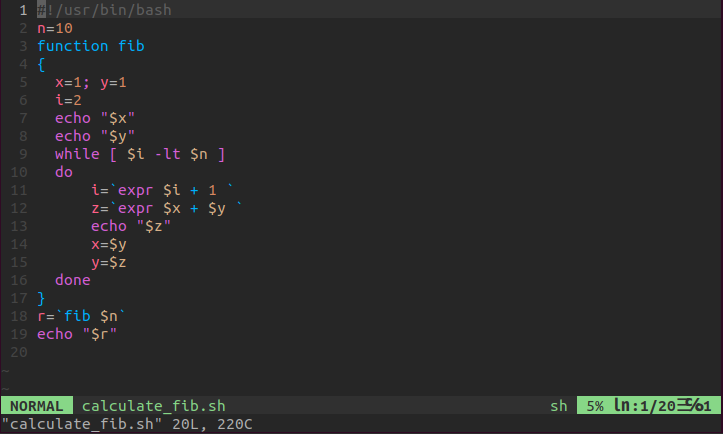
\includegraphics[width=4in]{chapters/part-1/figures/vim_fib.png}
	\caption{Vim (with user's profile customization as introduced in this chapter).}
\end{figure}

\begin{figure}[!htb]
	\centering
	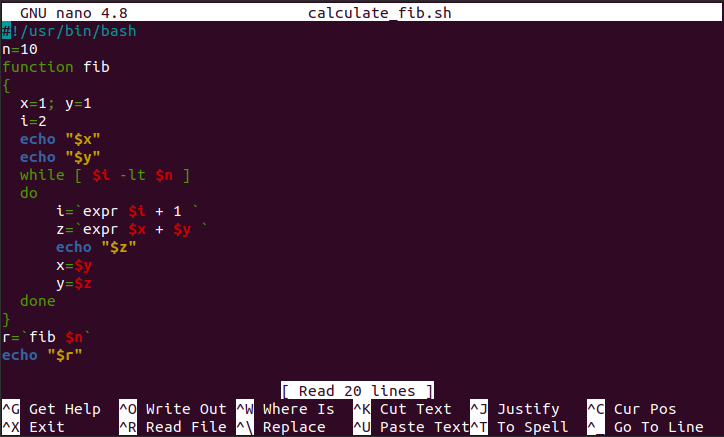
\includegraphics[width=4in]{chapters/part-1/figures/nano_fib.png}
	\caption{The nano editor.}
\end{figure}

\begin{figure}[!htb]
	\centering
	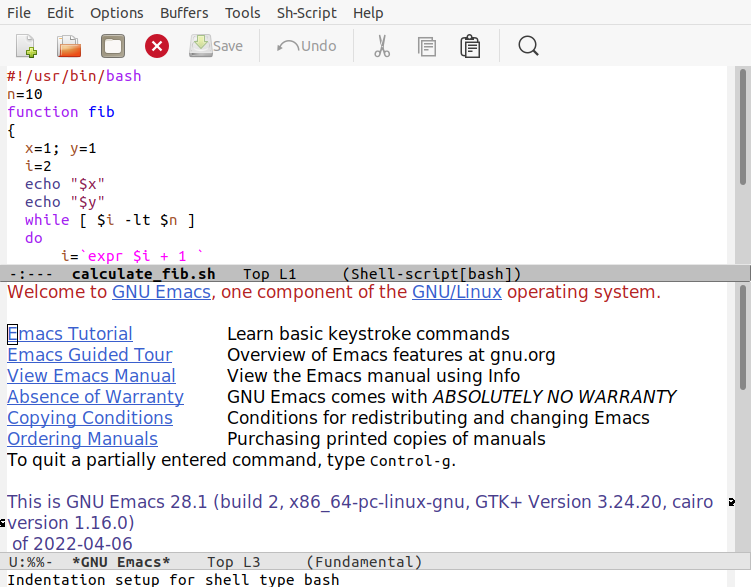
\includegraphics[width=4in]{chapters/part-1/figures/emacs_fib.png}
	\caption{The emacs editor.}
\end{figure}

\begin{figure}[!htb]
	\centering
	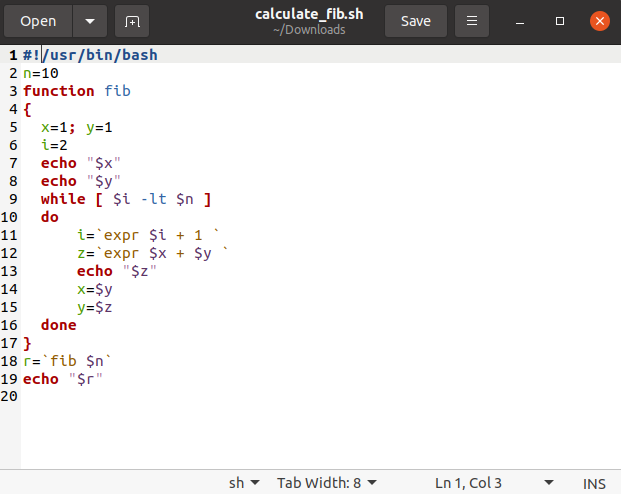
\includegraphics[width=4in]{chapters/part-1/figures/gedit_fib.png}
	\caption{The gedit editor.}
\end{figure}

\begin{figure}[!htb]
	\centering
	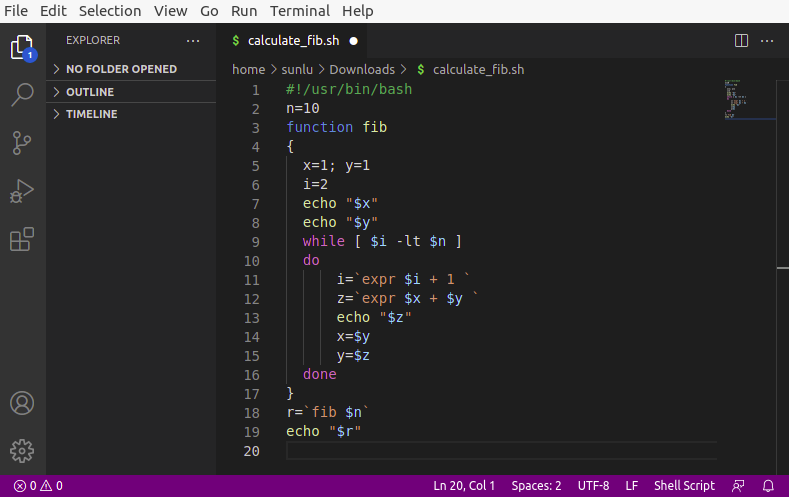
\includegraphics[width=4in]{chapters/part-1/figures/vscode_fib.png}
	\caption{Visual Studio Code.}
\end{figure}
